\documentclass[12pt]{article}
\usepackage[margin=2cm]{geometry}
\usepackage{amsmath}
\usepackage{slashed}
\usepackage{tikz}

\begin{document}

\noindent
Bhabha scattering is the result of interactions between positrons and electrons.
The following diagram represents a collider experiment with
collinear electron and positron beams.
\begin{center}
\begin{tikzpicture}
\draw[dashed] (0,0) circle (0.5cm);
\draw[thick,->] (2,0) node[anchor=west] {$e^-$} -- (0.6,0);
\draw[thick,->] (-2,0) node[anchor=east] {$e^+$} -- (-0.6,0);
\draw[thick,->] (0.40,0.40) -- (1.3,1.3) node[anchor=south west] {$e^+$};
\draw[thick,->] (-0.4,-0.4) -- (-1.3,-1.3) node[anchor=north east] {$e^-$};
\draw (1,0.5) node {$\theta$};
\end{tikzpicture}
\end{center}

\noindent
Here is the same diagram with momentum and spinor labels.

\begin{center}
\begin{tikzpicture}
\draw[dashed] (0,0) circle (0.5cm);
\draw[thick,->] (2,0) node[anchor=west] {$p_2, u_2$} -- (0.6,0);
\draw[thick,->] (-2,0) node[anchor=east] {$p_1, v_1$} -- (-0.6,0);
\draw[thick,->] (0.40,0.40) -- (1.3,1.3) node[anchor=south west] {$p_3, v_3$};
\draw[thick,->] (-0.4,-0.4) -- (-1.3,-1.3) node[anchor=north east] {$p_4, u_4$};
\draw (1,0.5) node {$\theta$};
\end{tikzpicture}
\end{center}

\noindent
In a typical collider experiment the momentum vectors are
\begin{equation*}
p_1=\begin{pmatrix}E\\0\\0\\p\end{pmatrix}\qquad
p_2=\begin{pmatrix}E\\0\\0\\-p\end{pmatrix}\qquad
p_3=\begin{pmatrix}
E\\
p\sin\theta\cos\phi\\
p\sin\theta\sin\phi\\
p\cos\theta
\end{pmatrix}
\qquad
p_4=\begin{pmatrix}
E\\
-p\sin\theta\cos\phi\\
-p\sin\theta\sin\phi\\
-p\cos\theta
\end{pmatrix}
\end{equation*}

\noindent
where $E=\sqrt{p^2+m^2}$.
The spinors are
\begin{gather*}
v_{11}=\begin{pmatrix}p\\0\\E+m\\0\end{pmatrix}\quad
u_{21}=\begin{pmatrix}E+m\\0\\-p\\0\end{pmatrix}\quad
v_{31}=\begin{pmatrix}p_3^z\\p_3^x+ip_3^y\\E+m\\0\end{pmatrix}\quad
u_{41}=\begin{pmatrix}E+m\\0\\p_4^z\\p_4^x+ip_4^y\end{pmatrix}
\\
v_{12}=\begin{pmatrix}0\\-p\\0\\E+m\end{pmatrix}\quad
u_{22}=\begin{pmatrix}0\\E+m\\0\\p\end{pmatrix}\quad
v_{32}=\begin{pmatrix}p_3^x-ip_3^y\\-p_3^z\\0\\E+m\end{pmatrix}\quad
u_{42}=\begin{pmatrix}0\\E+m\\p_4^x-ip_4^y\\-p_4^z\end{pmatrix}
\end{gather*}

\noindent
The spinors shown above are not individually normalized.
Instead, a combined spinor normalization constant $N=(E+m)^4$
will be used.

\bigskip
\noindent
This is the probability density for Bhabha scattering.
$$
|\mathcal{M}(s_1,s_2,s_3,s_4)|^2=\frac{e^4}{N}
\left|
-\frac{1}{t}(\bar{v}_1\gamma^\mu v_3)(\bar{u}_4\gamma_\mu u_2)
+\frac{1}{s}(\bar{v}_1\gamma^\nu u_2)(\bar{u}_4\gamma_\nu v_3)
\right|^2
$$

\noindent
Symbol $s_j$ selects the spin (up or down) of spinor $j$.
Symbol $e$ is electron charge.
Symbols $s$ and $t$ are Mandelstam variables $s=(p_1+p_2)^2$ and $t=(p_1-p_3)^2$.

\bigskip
\noindent
Let
\begin{equation*}
a_1=(\bar{v}_1\gamma^\mu v_3)(\bar{u}_4\gamma_\mu u_2)
\qquad
a_2=(\bar{v}_1\gamma^\nu u_2)(\bar{u}_4\gamma_\nu v_3)
\end{equation*}

\noindent
Then
\begin{align*}
|\mathcal{M}(s_1,s_2,s_3,s_4)|^2
&=
\frac{e^4}{N}\left|{-\frac{a_1}{t}} + \frac{a_2}{s}\right|^2\\
&=
\frac{e^4}{N}\left(-\frac{a_1}{t} + \frac{a_2}{s}\right)\left(-\frac{a_1}{t} + \frac{a_2}{s}\right)^*\\
&=
\frac{e^4}{N}
\left(
\frac{a_1a_1^*}{t^2} - \frac{a_1a_2^*}{st} -
\frac{a_1^*a_2}{st} + \frac{a_2a_2^*}{s^2}
\right)
\end{align*}

\noindent
The expected probability density $\langle|\mathcal{M}|^2\rangle$ is computed
by summing $|\mathcal{M}|^2$ over all spin states and dividing by the number of inbound states.
There are four inbound states.
\begin{align*}
\langle|\mathcal{M}|^2\rangle
&=
\frac{1}{4}\sum_{s_1=1}^2\sum_{s_2=1}^2\sum_{s_3=1}^2\sum_{s_4=1}^2
|\mathcal{M}(s_1,s_2,s_3,s_4)|^2\\
&=
\frac{e^4}{4}\sum_{s_1=1}^2\sum_{s_2=1}^2\sum_{s_3=1}^2\sum_{s_4=1}^2
\frac{1}{N}
\left(
\frac{a_1a_1^*}{t^2} - \frac{a_1a_2^*}{st} -
\frac{a_1^*a_2}{st} + \frac{a_2a_2^*}{s^2}
\right)
\end{align*}

\noindent
Use the Casimir trick to replace sums over spins with matrix products.
\begin{align*}
f_{11}&=\frac{1}{N}\sum_\text{spins}a_1a_1^*=
\mathop{\rm Tr}\left(
(\slashed{p}_1-m)\gamma^\mu(\slashed{p}_3-m)\gamma^\nu
\right)
\mathop{\rm Tr}\left(
(\slashed{p}_4+m)\gamma_\mu(\slashed{p}_2+m)\gamma_\nu
\right)
\\
f_{12}&=\frac{1}{N}\sum_{\rm spins}a_1a_2^*=
\mathop{\rm Tr}\left(
(\slashed{p}_1-m)\gamma^\mu(\slashed{p}_2+m)\gamma^\nu
(\slashed{p}_4+m)\gamma_\mu(\slashed{p}_3-m)\gamma_\nu
\right)
\\
f_{22}&=\frac{1}{N}\sum_\text{spins}a_2a_2^*=
\mathop{\rm Tr}\left(
(\slashed{p}_1-m)\gamma^\mu(\slashed{p}_2+m)\gamma^\nu
\right)
\mathop{\rm Tr}\left(
(\slashed{p}_4+m)\gamma_\mu(\slashed{p}_3-m)\gamma_\nu
\right)
\end{align*}

\noindent
Hence
\begin{equation*}
\langle|\mathcal{M}|^2\rangle
=\frac{e^4}{4}
\left(
\frac{f_{11}}{t^2} - \frac{f_{12}}{st} -
\frac{f_{12}^*}{st} + \frac{f_{22}}{s^2}
\right)
\end{equation*}

\noindent
Run ``bhabha-scattering-1.txt'' to verify the Casimir trick.

\bigskip
\noindent
The following momentum formulas are equivalent to the Casimir trick.
(Recall that $a\cdot b=a^\mu g_{\mu\nu}b^\nu$)
\begin{align*}
f_{11}&=
32(p_1\cdot p_2)(p_3\cdot p_4)+32(p_1\cdot p_4)(p_2\cdot p_3)
-32 m^2(p_1\cdot p_3)-32 m^2(p_2\cdot p_4)+64 m^4
\\
f_{12}&=
-32 (p_1\cdot p_4) (p_2\cdot p_3)
-16 m^2 (p_1\cdot p_2) + 16 m^2 (p_1\cdot p_3) - 16 m^2 (p_1\cdot p_4)\\
&\phantom{=}\qquad
{}- 16 m^2 (p_2\cdot p_3) + 16 m^2 (p_2\cdot p_4) - 16 m^2 (p_3\cdot p_4) - 32 m^4
\\
f_{22}&=
32(p_1\cdot p_3)(p_2\cdot p_4)+32(p_1\cdot p_4)(p_2\cdot p_3)
+32 m^2(p_1\cdot p_2)+32 m^2(p_3\cdot p_4)+64 m^4
\end{align*}

\noindent
In Mandelstam variables $s=(p_1+p_2)^2$, $t=(p_1-p_3)^2$, $u=(p_1-p_4)^2$ the formulas are
\begin{align*}
f_{11} &= 8 s^2 + 8 u^2 - 64 s m^2 - 64 u m^2 + 192 m^4
\\
f_{12} &= -8 u^2 + 64 u m^2 - 96 m^4
\\
f_{22} &= 8 t^2 + 8 u^2 - 64 t m^2 - 64 u m^2 + 192 m^4
\end{align*}

\subsection*{High energy approximation}
When $E\gg m$ a useful approximation is to set $m=0$ and obtain
\begin{align*}
f_{11}&= 8 s^2 + 8 u^2\\
f_{12}&= -8 u^2\\
f_{22}&= 8 t^2 + 8 u^2
\end{align*}

\noindent
For $m=0$ the Mandelstam variables are
\begin{align*}
s&=4E^2
\\
t&=-2E^2(1-\cos\theta)=-4E^2\sin^2(\theta/2)
\\
u&=-2E^2(1+\cos\theta)=-4E^2\cos^2(\theta/2)
\end{align*}

\noindent
It follows that
\begin{equation*}
s^2t^2=256E^8\sin^4(\theta/2)
\end{equation*}

\noindent
The corresponding expected probability density is
\begin{align*}
\langle|\mathcal{M}|^2\rangle
&=\frac{e^4}{4}
\left(
\frac{f_{11}}{t^2} - \frac{f_{12}}{st} -
\frac{f_{12}^*}{st} + \frac{f_{22}}{s^2}
\right)
\\
&=\frac{e^4}{4s^2t^2}
\left(
s^2f_{11}-stf_{12}-stf_{12}^*+t^2f_{22}
\right)
\\
&=\frac{e^4}{4s^2t^2}
\left(
s^2\left(8s^2+8u^2\right)+16stu^2+t^2\left(8t^2+8u^2\right)
\right)
\\
&=\frac{e^4}{1024E^8\sin^4(\theta/2)}
\left(
256E^8\cos^4\theta+1536E^8\cos^2\theta+2304E^8
\right)
\\
&=\frac{e^4}{4\sin^4(\theta/2)}
\left(\cos^4\theta+6\cos^2\theta+9\right)
\\
&=\frac{e^4}{4}
\frac{\left(\cos^2\theta+3\right)^2}{\sin^4(\theta/2)}
\end{align*}

\noindent
Run ``bhabha-scattering-2.txt'' to verify.

\subsection*{Cross section}
This is the differential cross section for Bhabha scattering.
\begin{equation*}
\frac{d\sigma}{d\Omega}
=\frac{\langle|\mathcal{M}|^2\rangle}{64\pi^2s}
=\frac{e^4}{1024\pi^2E^2}
\frac{\left(\cos^2\theta+3\right)^2}{\sin^4(\theta/2)}
\end{equation*}

\noindent
Substituting $e^4=16\pi^2\alpha^2$ yields
\begin{equation*}
\frac{d\sigma}{d\Omega}
=\frac{\alpha^2}{64E^2}
\frac{\left(\cos^2\theta+3\right)^2}{\sin^4(\theta/2)}
\end{equation*}

\noindent
We can integrate $d\sigma$ to obtain a cumulative distribution function.
Recall that
\begin{equation*}
d\Omega=\sin\theta\,d\theta\,d\phi
\end{equation*}

\noindent
Hence
\begin{equation*}
d\sigma=\frac{\alpha^2}{64E^2}
\frac{\left(\cos^2\theta+3\right)^2}{\sin^4(\theta/2)}\sin\theta\,d\theta\,d\phi
\end{equation*}

\bigskip
\noindent
Let $I(\theta)$ be the following integral of $d\sigma$.
\begin{align*}
I(\theta)
&=\left(\frac{64E^2}{\alpha^2}\right)\frac{1}{2\pi}
\int_0^{2\pi}\int d\sigma
\\
&=\int\frac{\left(\cos^2\theta+3\right)^2}{\sin^4(\theta/2)}\sin\theta\,d\theta,
\quad a\le\theta\le\pi
\end{align*}

\noindent
Angular support is limited to an arbitrary $a>0$ because $I(0)$ is undefined.
Assume $I(\theta)$ is computable by either symbolic or numerical integration.

\bigskip
\noindent
Let $C$ be the normalization constant
\begin{equation*}
C=I(\pi)-I(a)
\end{equation*}

\noindent
Then the cumulative distribution function $F(\theta)$ is
\begin{equation*}
F(\theta)=\frac{I(\theta)-I(a)}{C},
\quad a\le\theta\le\pi
\end{equation*}

\noindent
The probability of observing scattering events in the interval $\theta_1$ to $\theta_2$
can now be computed.
\begin{equation*}
P(\theta_1\le\theta\le\theta_2)=F(\theta_2)-F(\theta_1)
\end{equation*}

\noindent
Probability density function $f(\theta)$ is the derivative of $F(\theta)$.
\begin{equation*}
f(\theta)=\frac{dF(\theta)}{d\theta}
=\frac{1}{C}\frac{\left(\cos^2\theta+3\right)^2}{\sin^4(\theta/2)}\,\sin\theta
\end{equation*}

\noindent
Run ``bhabha-scattering-3.txt'' to draw $f(\theta)$ for $a=\pi/4=45^\circ$.

\begin{center}
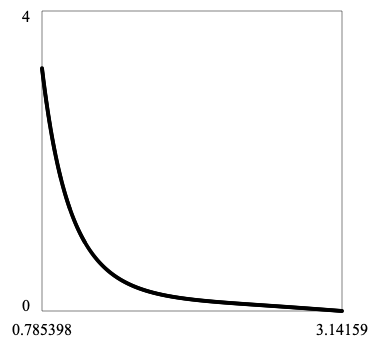
\includegraphics[scale=0.5]{bhabha-scattering.png}
\end{center}

\noindent
The following table shows the corresponding probability distribution for three bins.

\begin{center}
\begin{tabular}{|c|c|c|}
\hline
$\theta_1$ & $\theta_2$ & $P(\theta_1\le\theta\le\theta_2)$\\
\hline
$0^\circ$ & $45^\circ$ & -- \\
$45^\circ$ & $90^\circ$ & 0.83 \\
$90^\circ$ & $135^\circ$ & 0.13 \\
$135^\circ$ & $180^\circ$ & 0.04 \\
\hline
\end{tabular}
\end{center}

\noindent
Note: This is the closed form of $I(\theta)$.
\begin{equation*}
I(\theta)=-\frac{1}{3}\cos(3\theta)
-2\cos(2\theta)
-\frac{111}{3}\cos\theta
-\frac{32}{\sin^2(\theta/2)}
-128\log(\sin\theta),
\quad a\le\theta\le\pi
\end{equation*}

\subsection*{SLAC data}
\noindent
The following Bhabha scattering data is adapted from SLAC-PUB-1501.

\begin{center}
\begin{tabular}{|lr|c|c|}
\hline
& Bin & $x_k$, $x_{k+1}$ & $y$\\
\hline
(Smallest $\theta$) & 1 & $0.6, 0.5$ & 4432\\
& 2 & $0.5, 0.4$ & 2841\\
& 3 & $0.4, 0.3$ & 2045\\
& 4 & $0.3, 0.2$ & 1420\\
& 5 & $0.2, 0.1$ & 1136\\
& 6 & $0.1, 0.0$ & 852\\
& 7 & $0.0, -0.1$ & 656\\
& 8 & $-0.1, -0.2$ & 625\\
& 9 & $-0.2, -0.3$ & 511\\
& 10 & $-0.3, -0.4$ & 455\\
& 11 & $-0.4, -0.5$ & 402\\
(Largest $\theta$) & 12 & $-0.5, -0.6$ & 398\\
\hline
\end{tabular}
\end{center}

\noindent
Data column $y$ is the observed number of scattering events per bin.

\bigskip
\noindent
To compute predicted counts $\hat{y}$, integrate the probability density function
over each bin and multiply by the total number of observed counts.
\begin{equation*}
P_k=C^{-1}\int_{\arccos(x_k)}^{\arccos(x_{k+1})}
\frac{\left(\cos^2\theta+3\right)^2}{\sin^4(\theta/2)}\sin\theta
\end{equation*}
\begin{equation*}
\hat{y}_k=P_k\sum y
\end{equation*}

\noindent

\begin{center}
\begin{tabular}{|r|c|c|c|}
\hline
Bin & $x_k$, $x_{k+1}$ & $y$ & $\hat{y}$ \\
\hline
1 & $0.6, 0.5$ & 4432 & 4598\\
2 & $0.5, 0.4$ & 2841 & 2880\\
3 & $0.4, 0.3$ & 2045 & 1955\\
4 & $0.3, 0.2$ & 1420 & 1410\\
5 & $0.2, 0.1$ & 1136 & 1068\\
6 & $0.1, 0.0$ & 852 & 843\\
7 & $0.0, -0.1$ & 656 & 689\\
8 & $-0.1, -0.2$ & 625 & 582\\
9 & $-0.2, -0.3$ & 511 & 505\\
10 & $-0.3, -0.4$ & 455 & 450\\
11 & $-0.4, -0.5$ & 402 & 411\\
12 & $-0.5, -0.6$ & 398 & 382\\
\hline
\end{tabular}
\end{center}

\noindent
The coefficient of determination $R^2$ measures how well predicted values fit the real data.
Let $y$ be observed counts per bin and let $\hat{y}$ be predicted counts per bin.
Then
\begin{equation*}
R^2=1-\frac{\sum(y-\hat{y})^2}{\sum(y-\bar{y})^2}=0.997
\end{equation*}

\noindent
The result indicates that the model $\langle|\mathcal{M}|^2\rangle$ explains
99.7\% of the variance in the data.

\bigskip
\noindent
Run ``bhabha-scattering-4.txt'' to verify.

\subsection*{DESY data}
The following table shows DESY-PETRA Bhabha scattering data obtained from
HEP Data.\footnote{{\tt www.hepdata.net/record/ins191231} (Table 3, 14.0 GeV)}

\begin{center}
\begin{tabular}{|c|c|}
\hline
$x$ & $y$\\
\hline
$-0.73\phantom{00}$ & 0.10115\\
$-0.6495$ & 0.12235\\
$-0.5495$ & 0.11258\\
$-0.4494$ & 0.09968\\
$-0.3493$ & 0.14749\\
$-0.2491$ & 0.14017\\
$-0.149\phantom{0}$ & 0.1819\phantom{0}\\
$-0.0488$ & 0.22964\\
$\phantom{+}0.0514$ & 0.25312\\
$\phantom{+}0.1516$ & 0.30998\\
$\phantom{+}0.252\phantom{0}$ & 0.40898\\
$\phantom{+}0.3524$ & 0.62695\\
$\phantom{+}0.4529$ & 0.91803\\
$\phantom{+}0.5537$ & 1.51743\\
$\phantom{+}0.6548$ & 2.56714\\
$\phantom{+}0.7323$ & 4.30279\\
\hline
\end{tabular}
\end{center}

\noindent
Data $x$ and $y$ have the following relationship
with the cross section model.
\begin{equation*}
x=\cos\theta
\qquad
y=\frac{d\sigma}{d\Omega}
\end{equation*}

\noindent
The differential cross section for Bhabha scattering is
\begin{equation*}
\frac{d\sigma}{d\Omega}
=\frac{\langle|\mathcal{M}|^2\rangle}{64\pi^2s}
=\frac{\alpha^2}{2s}
\left(\frac{s^2+u^2}{t^2}+\frac{2u^2}{st}+\frac{t^2+u^2}{s^2}\right)
\end{equation*}

\noindent
The predicted cross section $\hat{y}$ is computed from data $x$ and beam energy $E$ as
\begin{equation*}
\hat{y}
=\frac{\alpha^2}{2s}
\left(\frac{s^2+u^2}{t^2}+\frac{2u^2}{st}+\frac{t^2+u^2}{s^2}\right)
\times(\hbar c)^2
\times10^{37}
\end{equation*}

\noindent
where
\begin{align*}
s&=4E^2
\\
t&=-2E^2(1-x)
\\
u&=-2E^2(1+x)
\end{align*}

\noindent
Factor $(\hbar c)^2$ converts the result to SI and factor $10^{37}$ converts square meters to nanobarns.

\bigskip
\noindent
The following table shows $\hat{y}$ for $E=7.0\,\text{GeV}$.

\begin{center}
\begin{tabular}{|c|c|c|}
\hline
$x$ & $y$ & $\hat{y}$\\
\hline
$-0.73\phantom{00}$ & 0.10115 & 0.110296\\
$-0.6495$ & 0.12235 & 0.113816\\
$-0.5495$ & 0.11258 & 0.120101\\
$-0.4494$ & 0.09968 & 0.129075\\
$-0.3493$ & 0.14749 & 0.141592\\
$-0.2491$ & 0.14017 & 0.158934\\
$-0.149\phantom{0}$ & 0.1819\phantom{0} & 0.182976\\
$-0.0488$ & 0.22964 & 0.216737\\
$\phantom{+}0.0514$ & 0.25312 & 0.264989\\
$\phantom{+}0.1516$ & 0.30998 & 0.335782\\
$\phantom{+}0.252\phantom{0}$ & 0.40898 & 0.44363\phantom{0}\\
$\phantom{+}0.3524$ & 0.62695 & 0.615528\\
$\phantom{+}0.4529$ & 0.91803 & 0.9077\phantom{00}\\
$\phantom{+}0.5537$ & 1.51743 & 1.45175\phantom{0}\\
$\phantom{+}0.6548$ & 2.56714 & 2.60928\phantom{0}\\
$\phantom{+}0.7323$ & 4.30279 & 4.61509\phantom{0}\\
\hline
\end{tabular}
\end{center}

\noindent
The coefficient of determination $R^2$ measures how well predicted values fit the real data.
\begin{equation*}
R^2=1-\frac{\sum(y-\hat{y})^2}{\sum(y-\bar{y})^2}=0.995
\end{equation*}

\noindent
The result indicates that the model $d\sigma$ explains 99.5\% of the variance in the data.

\bigskip
\noindent
Run ``bhabha-scattering-5.txt'' to verify.

\subsection*{Notes on Eigenmath scripts}
Here are a few notes about how the Eigenmath scripts work.
In component notation the trace operators of the Casimir trick become sums over the repeated index $\alpha$.
\begin{align*}
f_{11}&=
\left(
(\slashed{p}_1-m)^\alpha{}_\beta
\gamma^{\mu\beta}{}_\rho
(\slashed{p}_3-m)^\rho{}_\sigma
\gamma^{\nu\sigma}{}_\alpha
\right)
\left(
(\slashed{p}_4+m)^\alpha{}_\beta
\gamma_\mu{}^\beta{}_\rho
(\slashed{p}_2+m)^\rho{}_\sigma
\gamma_\nu{}^\sigma{}_\alpha
\right)
\\
f_{12}&=
(\slashed{p}_1-m)^\alpha{}_\beta
\gamma^{\mu\beta}{}_\rho
(\slashed{p}_2+m)^\rho{}_\sigma
\gamma^{\nu\sigma}{}_\tau
(\slashed{p}_4+m)^\tau{}_\delta
\gamma_\mu{}^\delta{}_\eta
(\slashed{p}_3-m)^\eta{}_\xi
\gamma_\nu{}^\xi{}_\alpha
\\
f_{22}&=
\left(
(\slashed{p}_1-m)^\alpha{}_\beta
\gamma^{\mu\beta}{}_\rho
(\slashed{p}_2+m)^\rho{}_\sigma
\gamma^{\nu\sigma}{}_\alpha
\right)
\left(
(\slashed{p}_4+m)^\alpha{}_\beta
\gamma_\mu{}^\beta{}_\rho
(\slashed{p}_3-m)^\rho{}_\sigma
\gamma_\nu{}^\sigma{}_\alpha
\right)
\end{align*}

\noindent
To convert the above formulas to Eigenmath code,
the $\gamma$ tensors need to be transposed
so that repeated indices are adjacent to each other.
Also, multiply $\gamma^\mu$ by the metric tensor to lower the index.
\begin{align*}
\gamma^{\beta\mu}{}_\rho\quad&\rightarrow\quad
\text{\tt gammaT = transpose(gamma)}\\
\gamma^\beta{}_{\mu\rho}\quad&\rightarrow\quad
\text{\tt gammaL = transpose(dot(gmunu,gamma))}
\end{align*}

\noindent
Define the following $4\times4$ matrices.
\begin{align*}
(\slashed{p}_1-m)\quad&\rightarrow\quad\text{\tt X1 = pslash1 - m I}\\
(\slashed{p}_2+m)\quad&\rightarrow\quad\text{\tt X2 = pslash2 + m I}\\
(\slashed{p}_3-m)\quad&\rightarrow\quad\text{\tt X3 = pslash3 - m I}\\
(\slashed{p}_4+m)\quad&\rightarrow\quad\text{\tt X4 = pslash4 + m I}
\end{align*}

\noindent
Then for $f_{11}$ we have the following Eigenmath code.
The contract function sums over $\alpha$.
\begin{align*}
(\slashed{p}_1-m)^\alpha{}_\beta
\gamma^{\mu\beta}{}_\rho
(\slashed{p}_3-m)^\rho{}_\sigma
\gamma^{\nu\sigma}{}_\alpha
\quad&\rightarrow\quad
\text{\tt T1 = contract(dot(X1,gammaT,X3,gammaT),1,4)}\\
(\slashed{p}_4+m)^\alpha{}_\beta
\gamma_\mu{}^\beta{}_\rho
(\slashed{p}_2+m)^\rho{}_\sigma
\gamma_\nu{}^\sigma{}_\alpha
\quad&\rightarrow\quad
\text{\tt T2 = contract(dot(X4,gammaL,X2,gammaL),1,4)}
\end{align*}

\noindent
Next, multiply then sum over repeated indices.
The dot function sums over $\nu$ then the contract function
sums over $\mu$. The transpose makes the $\nu$ indices adjacent
as required by the dot function.
$$
f_{11}=
\mathop{\rm Tr}(\cdots\gamma^\mu\cdots\gamma^\nu)
\mathop{\rm Tr}(\cdots\gamma_\mu\cdots\gamma_\nu)
\quad\rightarrow\quad
\text{\tt f11 = contract(dot(T1,transpose(T2)))}
$$

\noindent
Follow suit for $f_{22}$.
\begin{align*}
(\slashed{p}_1-m)^\alpha{}_\beta
\gamma^{\mu\beta}{}_\rho
(\slashed{p}_2+m)^\rho{}_\sigma
\gamma^{\nu\sigma}{}_\alpha
\quad&\rightarrow\quad
\text{\tt T1 = contract(dot(X1,gammaT,X2,gammaT),1,4)}
\\
(\slashed{p}_4+m)^\alpha{}_\beta
\gamma_\mu{}^\beta{}_\rho
(\slashed{p}_3-m)^\rho{}_\sigma
\gamma_\nu{}^\sigma{}_\alpha
\quad&\rightarrow\quad
\text{\tt T2 = contract(dot(X4,gammaL,X3,gammaL),1,4)}
\end{align*}

\noindent
Hence
$$
f_{22}=
\mathop{\rm Tr}(\cdots\gamma^\mu\cdots\gamma^\nu)
\mathop{\rm Tr}(\cdots\gamma_\mu\cdots\gamma_\nu)
\quad\rightarrow\quad
\text{\tt f22 = contract(dot(T1,transpose(T2)))}
$$

\noindent
The calculation of $f_{12}$ begins with
\begin{multline*}
(\slashed{p}_1-m)^\alpha{}_\beta
\gamma^{\mu\beta}{}_\rho
(\slashed{p}_2+m)^\rho{}_\sigma
\gamma^{\nu\sigma}{}_\tau
(\slashed{p}_4+m)^\tau{}_\delta
\gamma_\mu{}^\delta{}_\eta
(\slashed{p}_3-m)^\eta{}_\xi
\gamma_\nu{}^\xi{}_\alpha
\\
\rightarrow\quad
\text{\tt T = contract(dot(X1,gammaT,X2,gammaT,X4,gammaL,X3,gammaL),1,6)}
\end{multline*}

\noindent
Then sum over repeated indices $\mu$ and $\nu$.
$$
f_{12}=\mathop{\rm Tr}(\cdots\gamma^\mu\cdots\gamma^\nu\cdots\gamma_\mu\cdots\gamma_\nu)
\quad\rightarrow\quad
\text{\tt f12 = contract(contract(T,1,3))}
$$

%F(theta) = -37/8 cos(theta) - 1/4 cos(2 theta) - 1/24 cos(3 theta) - 4 / sin(theta/2)^2 - 16 log(sin(theta/2))

%\subsection*{Epilogue}
%This is the closed form of $I(\theta)$.
%\begin{equation*}
%I(\theta)=-\tfrac{37}{8}\cos\theta - \tfrac{1}{4}\cos(2\theta)
%- \tfrac{1}{24}\cos(3\theta) - \frac{4}{\sin(\theta/2)^2} - 16\log(\sin(\theta/2))
%\end{equation*}

\end{document}
